%----------------------------------------------------------------------------------------
%	PACKAGES AND OTHER DOCUMENT CONFIGURATIONS
%----------------------------------------------------------------------------------------

\documentclass[12pt]{article}

\usepackage{amsmath}
\usepackage{caption}
\usepackage[colorinlistoftodos]{todonotes}
\usepackage[english]{babel}
\usepackage{graphicx}
\usepackage{hyperref}
\usepackage{subcaption}
\usepackage[utf8x]{inputenc}
\usepackage{yfonts,color}

\setlength\parindent{24pt}

%----------------------------------------------------------------------------------------
%	BEGIN TITLE PAGE
%----------------------------------------------------------------------------------------

\begin{document}

\begin{titlepage}
\newcommand{\HRule}{\rule{\linewidth}{0.5mm}}
\center

\textsc{\LARGE The University of Akron}\\[1.5cm]
\textsc{\Large Senior Design}\\[0.5cm]
\textsc{\large Hydrophone Pinger Locator}\\[0.5cm]

\HRule \\[0.4cm]
{ \huge \bfseries TDOA Location Algorithm}\\[0.4cm]
\HRule \\[1.5cm]

\begin{minipage}{0.4\textwidth}
\begin{flushleft} \large
\emph{Authors:}\\
Michael \textsc{Daub}\newline
Zachary \textsc{Goyetche}\newline
Joshua \textsc{Simmons}\newline
Shane \textsc{Stroh}
\end{flushleft}
\end{minipage}
~
\begin{minipage}{0.4\textwidth}
\begin{flushright} \large
\emph{Supervisor:} \\
Dr. Ryan \textsc{Toonen}
\end{flushright}
\end{minipage}\\[2cm]

{\large \today}\\[0.5cm]


\includegraphics[width=5.0cm]{/Users/betio32/Documents/myGitHub/Senior-Design/Reports/Pics_and_Figs/UA_Seal.png}

\vfill

\end{titlepage}

%----------------------------------------------------------------------------------------
%	BEGIN TABLE OF CONTENTS
%----------------------------------------------------------------------------------------

\renewcommand*\contentsname{Summary}
\tableofcontents
\pagebreak

%----------------------------------------------------------------------------------------
%	BEGIN MAIN BODY OF DOCUMENT
%----------------------------------------------------------------------------------------

\section{TDOA}

\subsection{Pseudo-Doppler vs. TDOA}

%yinipar{\color{blue}P}{seudo-Doppler} 
Pseudo-Doppler takes advantage of the \href{<http://www.dailymotion.com/video/x1h5ogx_carl-sagan-s-cosmos-e10-the-edge-of-forever_tv>}{Doppler Effect.} Imagine rotating an antenna at high speed in a circle. As the antenna swings towards the source, the induced SINE wave (Doppler tone) will blue shift. When the antenna swings away from the source, the Doppler tone will red shift. The point where the phase crosses the x-axis is when the antenna is in alignment with the source.\\

\begin{figure}[!h]
	\centering
	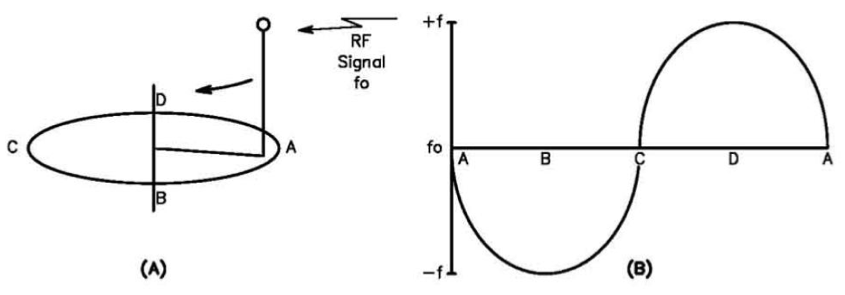
\includegraphics[width=10.0cm]{/Users/betio32/Documents/myGitHub/Senior-Design/Reports/Pics_and_Figs/Pseudo_Doppler_Theory_of_Operation.png}
    \caption{Pseudo-doppler theory of operation.} \label{fig:Doppler Theory of Operation}
\end{figure}

\noindent The rotational speed required for the antenna can be determined using the following equation.

\[\omega = \frac{v_p  \Delta f}{r f_c}\]

\begin{center}
\begin{tabular}{l}
$\omega$ = Angular Velocity $[$ rad/s $]$\\
$v_p$ = Phase Velocity $[$ m/s $]$\\
$\Delta f$ = Doppler Tone Frequency $[$ Hz $]$\\
r = Moment Arm Radius $[$ m $]$\\
$f_c$ = Carrier Frequency $[$ Hz $]$\\
\end{tabular}
\end{center}

\noindent For a phase velocity of 1482 m/s, a desired Doppler tone of 500 Hz, a moment arm radius of 5 cm, and a carrier frequency of 30 kHz; this would require an angular velocity of 494 rad/s or 4717 RPM!

\pagebreak

\noindent Because the RPM requirement is so high, the rotating antenna is imitated by the  consecutive sampling of several stationary antenna in a circular pattern; this is termed "Pseudo-Doppler".

\vspace{5mm}
    
\begin{figure}[!h]
	\centering
	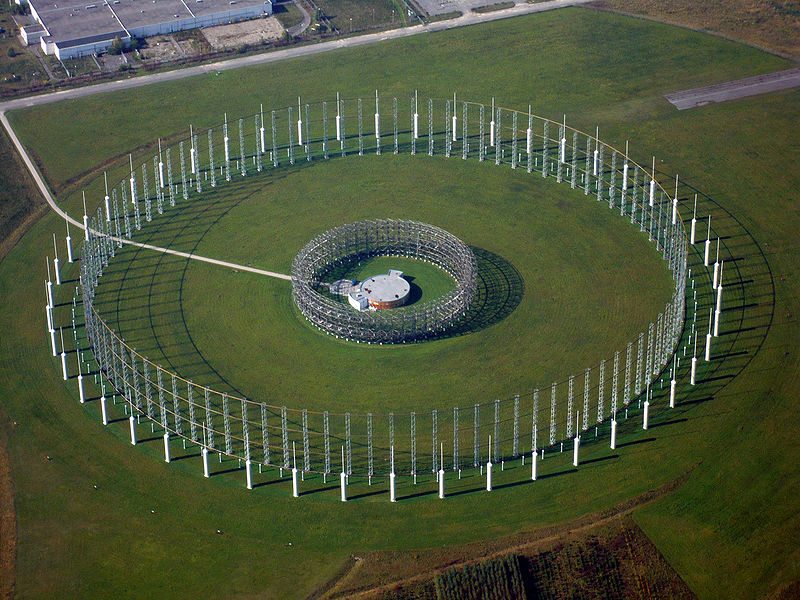
\includegraphics[width=10.0cm]{/Users/betio32/Documents/myGitHub/Senior-Design/Reports/Pics_and_Figs/Pseudo_Doppler_Antennae_Array.png}
    \caption{Pseudo-doppler antennae array.} \label{fig:Doppler Array}
\end{figure}

\noindent Pseudo-Doppler is a very popular technique among fox hunters (type of HAM radio user) for finding the location of RF sources. However, the major drawback of Pseudo-Doppler is that it only provides an azimuth angle to the direction of the source. Another directional finding algorithm will need to be implemented in order to provide both an azimuth angle and an elevation angle.\\

\noindent Time-Difference-of-Arrival (TDOA) is the algorithm of choice for providing the desired azimuth information to a source in 3D space. It utilizes the time delay of the received signal from multiple sensors for locating the source.\\

\noindent An excellent example to demonstrate TDOA is the Global Positioning System (GPS). Eve is an geocaching enthusiast. She needs to determine her location on the Earths surface to a high degree of precision. She reaches into her backpack and retrieves her GPS. After turning it on, it broadcasts a time stamped RF signal isotropically in all directions. The RF signal leaves Earths atmosphere and into outer space where it is picked up by a GPS satellite. After a short while, three other GPS satellites begin receiving the RF signal. Each satellite can determine the signal time-of-arrival (TOA) by taking the difference in time between the atomic clock in the satellite and the time stamp embedded in the signal. Once the TOAs have been calculated, the TOAs are multiplied by the speed of light producing segments of different length. Eve's position can then be determined through triangulation.\\

\noindent The process by which a signal is located based on the measurement of the difference in distances between the reception of a broadcasted signal at two or more receivers at known times is called multilateration. Such mathematical problems involve determining the intersection of spherical shells.
    
\subsection{Diamond Geometry Mathematical Derivation}
\begin{figure}[!h]
	\centering
	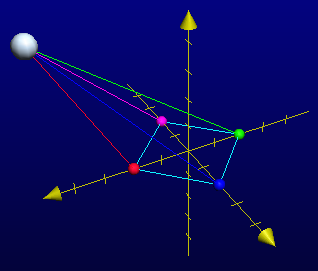
\includegraphics[width=10.0cm]{/Users/betio32/Documents/myGitHub/Senior-Design/Reports/Pics_and_Figs/TDOA_Diamond_Visual.png}
    \caption{TDOA diamond setup.} \label{fig:TDOA Diamond Visual}
\end{figure}  

\pagebreak
\noindent Assume the source is an isotropic radiator. Referring to Figure 3, the source is the white dot, chan1 is the blue dot, chan2 is the red dot, chan3 is the magenta dot, and chan4 is the green dot. The radii from source to chan are also color coded correctly.\\

\noindent The radii have length proportional to $v_p$ and the respective TOA for each channel.

\begin{center}
\begin{tabular}{l}
$R_1 = v_p TOA_1$\\
$R_2 = v_p TOA_2$\\
$R_3 = v_p TOA_3$\\
$R_4 = v_p TOA_4$\\
\end{tabular}
\end{center}

\noindent Using channel 1 as the reference, the radii can be re-written as the following where $tD$ denotes the time delay.

\begin{center}
\begin{tabular}{l}
$R_1 = v_p TOA_1$\\
$R_2 = v_p (TOA_1 - tD_2)$\\
$R_3 = v_p (TOA_1 - tD_3)$\\
$R_4 = v_p (TOA_1 - tD_4)$\\
\end{tabular}
\end{center}

\noindent The coordinates for all of the dots are

\begin{center}
\begin{tabular}{l}
$S = (x_s,y_s,z_s)$\\
$C_1 = (0,D,0)$\\
$C_2 = (D,0,0)$\\
$C_3 = (0,-D,0)$\\
$C_4 = (-D,0,0)$\\
\end{tabular}
\end{center}

\noindent Constructing vectors from the channels to the source

\begin{center}
\begin{tabular}{l}
$\overrightarrow{R_1} = (x_s,y_s-D,z_s)$\\
$\overrightarrow{R_2} = (x_s-D,y_s,z_s)$\\
$\overrightarrow{R_3} = (x_s,y_s+D,z_s)$\\
$\overrightarrow{R_4} = (x_s+D,y_s,z_s)$\\
\end{tabular}
\end{center}

\pagebreak
\noindent The square of the magnitude of the radii vectors are

\begin{center}
\begin{equation} \label{eq:1}
(R_1)^2 = (x_s)^2 + (y_s-D)^2 + (z_s)^2
\end{equation}
\begin{equation} \label{eq:2}
(R_2)^2 = (x_s-D)^2 + (y_s)^2 + (z_s)^2
\end{equation}
\begin{equation} \label{eq:3}
(R_3)^2 = (x_s)^2 + (y_s+D)^2 + (z_s)^2
\end{equation}
\begin{equation} \label{eq:4}
(R_4)^2 = (x_s+D)^2 + (y_s)^2 + (z_s)^2
\end{equation}
\end{center}

\vspace{4 mm}
\noindent Which can be expressed alternatively as\\

\begin{center}
\begin{equation} \label{eq:5}
(R_1)^2 = (v_p TOA_1)^2
\end{equation}
\begin{equation} \label{eq:6}
(R_2)^2 = [v_p (TOA_1 + tD_2)]^2
\end{equation}
\begin{equation} \label{eq:7}
(R_3)^2 = [v_p (TOA_1 + tD_3)]^2
\end{equation}
\begin{equation} \label{eq:8}
(R_4)^2 = [v_p (TOA_1 + tD_4)]^2
\end{equation}
\end{center}

\vspace{5 mm}
\noindent Subtracting Eq. 1 from Eq. 3 yields
\begin{center}
\begin{equation} \label{eq:10}
y_s = \frac{(R_3)^2 - (R_1)^2}{4D}
\end{equation}
\end{center}

\pagebreak
\noindent Subtracting Eq. 2 from Eq. 4 yields similarly
\begin{center}
\begin{equation} \label{eq:11}
x_s = \frac{(R_4)^2 - (R_2)^2}{4D}
\end{equation}
\end{center}

\noindent Use Eq. 1 to find z
\begin{center}
\begin{equation} \label{eq:12}
z_s \pm \sqrt[]{(R_1)^2 - (x_s)^2 - (y_s-D)^2}
\end{equation}
\end{center}

\vspace{5 mm}
\noindent We see that z has two possible solutions. By inspection

\begin{center}
\begin{equation} \label{eq:9}
(R_1)^2 + (R_3)^2 = (R_2)^2 + (R_4)^2
\end{equation}
\end{center}

\begin{center}
\begin{tabular}{l}
$ (x_s)^2   + (y_s-D)^2 + (z_s)^2 + (x_s)^2   + (y_s+D)^2 + (z_s)^2 \stackrel{?}{=}$\\
$ (x_s-D)^2 + (y_s)^2   + (z_s)^2 + (x_s+D)^2 + (y_s)^2   + (z_s)^2$\\
\\
$ 2(x_s)^2 + 2(y_s)^2 + 2(z_s)^2 + 2(D)^2 = 2(x_s)^2 + 2(y_s)^2 + 2(z_s)^2 + 2(D)^2$\\
\end{tabular}
\end{center}

\vspace{5 mm}
\noindent Substituting Eq. 5, Eq. 6, Eq. 7, and Eq. 8 into Eq. 9 yields.
\begin{center}
\begin{equation} \label{eq:13}
TOA_1 = \frac{(tD_2)^2+(tD_4)^2-(tD_3)^2}{2(tD_3-tD_2-tD_4)}
\end{equation}
\end{center}

\pagebreak

\subsection{Tetrahedron Geometry Mathematical Derivation}
\begin{figure}[!h]
	\centering
	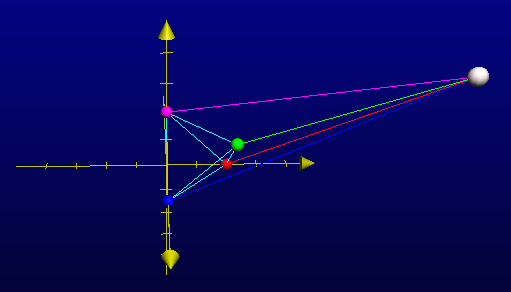
\includegraphics[width=10.0cm]{/Users/betio32/Documents/myGitHub/Senior-Design/Reports/Pics_and_Figs/TDOA_Tetrahedron_Visual.png}
    \caption{TDOA tetrahedron setup.} \label{fig:TDOA Tetrahedron Visual}
\end{figure} 

\noindent The diamond configuration contains ambiguity as to the location of the source because the sensors all lie in the same plane. To mitigate this, the tetrahedron geometry was explored. It is the simplest 3D geometric shape.

\noindent The derivation follows similarly as before. Assume the source is an isotropic radiator. Referring to Figure 4, the source is the white dot, chan1 is the blue dot, chan2 is the red dot, chan3 is the magenta dot, and chan4 is the green dot. The radii from source to chan are also color coded correctly.\\

\noindent The radii have length proportional to $v_p$ and the respective TOA for each channel.

\begin{center}
\begin{tabular}{l}
$R_1 = v_p TOA_1$\\
$R_2 = v_p TOA_2$\\
$R_3 = v_p TOA_3$\\
$R_4 = v_p TOA_4$\\
\end{tabular}
\end{center}

\noindent Using channel 1 as the reference, the radii can be re-written as the following where $tD$ denotes the time delay.

\begin{center}
\begin{tabular}{l}
$R_1 = v_p TOA_1$\\
$R_2 = v_p (TOA_1 - tD_2)$\\
$R_3 = v_p (TOA_1 - tD_3)$\\
$R_4 = v_p (TOA_1 - tD_4)$\\
\end{tabular}
\end{center}

\pagebreak
\noindent The coordinates for all of the dots are

\begin{center}
\begin{tabular}{l}
$S = (x_s,y_s,z_s)$\\
$C_1 = (D,0,0)$\\
$C_2 = (0,D,0)$\\
$C_3 = (0,0,D)$\\
$C_4 = (D,D,D)$\\
\end{tabular}
\end{center}

\noindent Constructing vectors from the channels to the source

\begin{center}
\begin{tabular}{l}
$\overrightarrow{R_1} = (x_s-D,y_s,z_s)$\\
$\overrightarrow{R_2} = (x_s,y_s-D,z_s)$\\
$\overrightarrow{R_3} = (x_s,y_s,z_s-D)$\\
$\overrightarrow{R_4} = (x_s-D,y_s-D,z_s-D)$\\
\end{tabular}
\end{center}

\noindent The square of the magnitude of the radii vectors are

\begin{center}
\begin{equation} \label{eq:14}
(R_1)^2 = (x_s-D)^2 + (y_s)^2 + (z_s)^2
\end{equation}
\begin{equation} \label{eq:15}
(R_2)^2 = (x_s)^2 + (y_s-D)^2 + (z_s)^2
\end{equation}
\begin{equation} \label{eq:16}
(R_3)^2 = (x_s)^2 + (y_s)^2 + (z_s-D)^2
\end{equation}
\begin{equation} \label{eq:17}
(R_4)^2 = (x_s-D)^2 + (y_s-D)^2 + (z_s-D)^2
\end{equation}
\end{center}

\vspace{5 mm}
\noindent Which can be expressed alternatively as

\begin{center}
\begin{equation} \label{eq:18}
(R_1)^2 = (v_p TOA_1)^2
\end{equation}
\begin{equation} \label{eq:19}
(R_2)^2 = [v_p (TOA_1 + tD_2)]^2
\end{equation}
\begin{equation} \label{eq:20}
(R_3)^2 = [v_p (TOA_1 + tD_3)]^2
\end{equation}
\begin{equation} \label{eq:21}
(R_4)^2 = [v_p (TOA_1 + tD_4)]^2
\end{equation}
\end{center}

\pagebreak

\noindent Use Eq. 14 and Eq. 15
\begin{center}
\begin{equation} \label{eq:22}
y_s = \frac{(R_1)^2 - (R_2)^2 - 2Dx_s}{2D}
\end{equation}
\end{center}

\vspace{5 mm}
\noindent Use Eq. 16 and Eq. 17
\begin{center}
\begin{equation} \label{eq:23}
y_s = \frac{(R_3)^2 - (R_4)^2 + 2(D)^2 - 2Dx_s}{2D}
\end{equation}
\end{center}

\vspace{5 mm}
\noindent Use Eq. 22 and Eq. 23 
\begin{center}
\begin{equation} \label{eq:24}
x_s = \frac{-(R_1)^2 + (R_2)^2 + (R_3)^2 - (R_4)^2 + 2(D)^2}{4D}
\end{equation}
\end{center}

\vspace{5 mm}
\noindent Use Eq. 24 and Eq. 22
\begin{center}
\begin{equation} \label{eq:25}
y_s = \frac{(R_1)^2 - (R_2)^2 + (R_3)^2 - (R_4)^2 + 2(D)^2}{4D}
\end{equation}
\end{center}

\vspace{5 mm}
\noindent Subtract Eq. 1 from Eq. 4
\begin{center}
\begin{equation} \label{eq:26}
z_s = \frac{(R_1)^2 - (R_4)^2 + -2Dy_s + 2(D)^2}{2D}
\end{equation}
\end{center}

\vspace{5 mm}
\noindent Use Eq. 26 and Eq. 25
\begin{center}
\begin{equation} \label{eq:27}
z_s = \frac{(R_1)^2 + (R_2)^2 - (R_3)^2 - (R_4)^2 + 2(D)^2}{4D}
\end{equation}
\end{center}

\pagebreak
\noindent Use Eq. 24, Eq. 25, and Eq. 27
\begin{center}
\begin{equation} \label{eq:28}
\begin{split}
0 &= [-(R_1)^2+(R_2)^2+(R_3)^2-(R_4)^2-2(D)^2]^2 \\
  &+ [ (R_1)^2-(R_2)^2+(R_3)^2-(R_4)^2+2(D)^2]^2 \\
  &+ [ (R_1)^2+(R_2)^2-(R_3)^2-(R_4)^2+2(D)^2]^2 \\
  &- 16(DR_1)^2
\end{split}
\end{equation}
\end{center}

\noindent We note that there is no closed form solution for finding $R_1$ and thus $TOA_1$. To solve for $TOA_1$ a root-finding algorithm will have to be used (Eg. Bisector Method).

\subsection{Using Cross-Correlation for Determining the Time Delays}

\vspace{5 mm}
\noindent The cross-correlation function is defined as
\begin{center}
\begin{equation} \label{eq:29}
\Psi_\tau (t) = \int_{}^{} y_1(t) y_2(t-\tau) dt
\end{equation}
\end{center}

\vspace{5 mm}
\noindent Where $y_1$ and $y_2$ are energy signals.

\begin{figure}[!h]
	\centering
	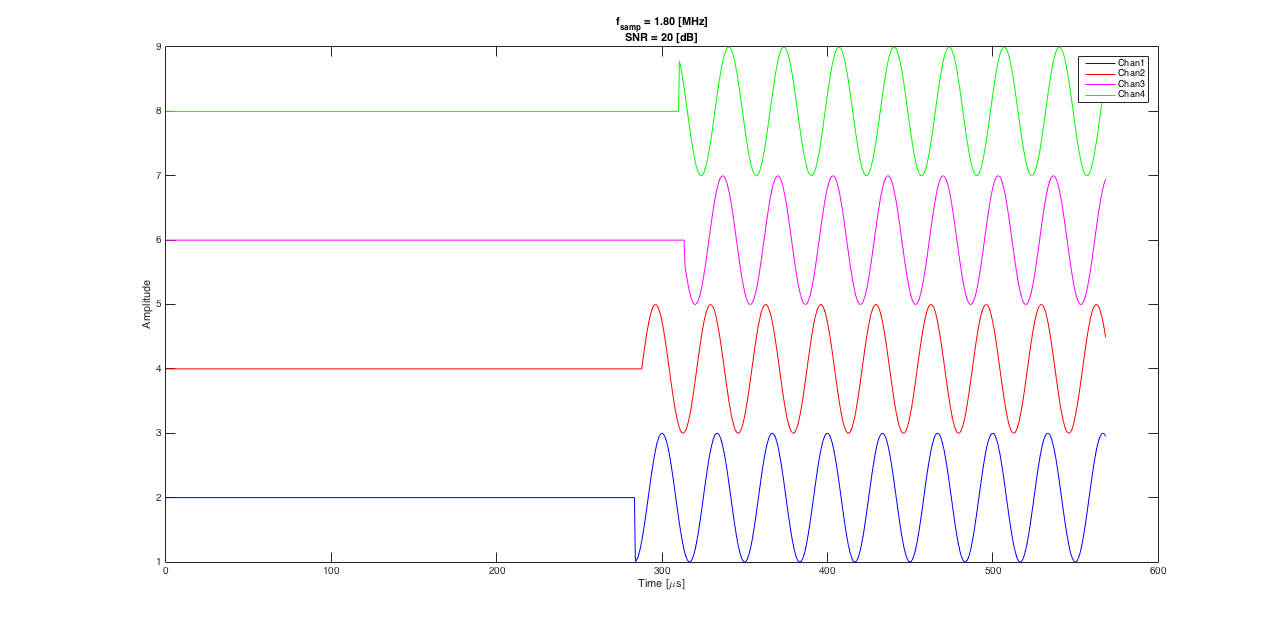
\includegraphics[width=10.0cm]{/Users/betio32/Documents/myGitHub/Senior-Design/Reports/Pics_and_Figs/Delayed_Sines_Heads.png}
    \caption{Time delayed sines for TDOA.} \label{fig:Delayed_Sines_Heads}
\end{figure}

\pagebreak
\noindent Referring to Fig. 5, applying the cross-correlation function to chan2 using chanl 1 as the reference yields Fig. 6.

\begin{figure}[!h]
	\centering
	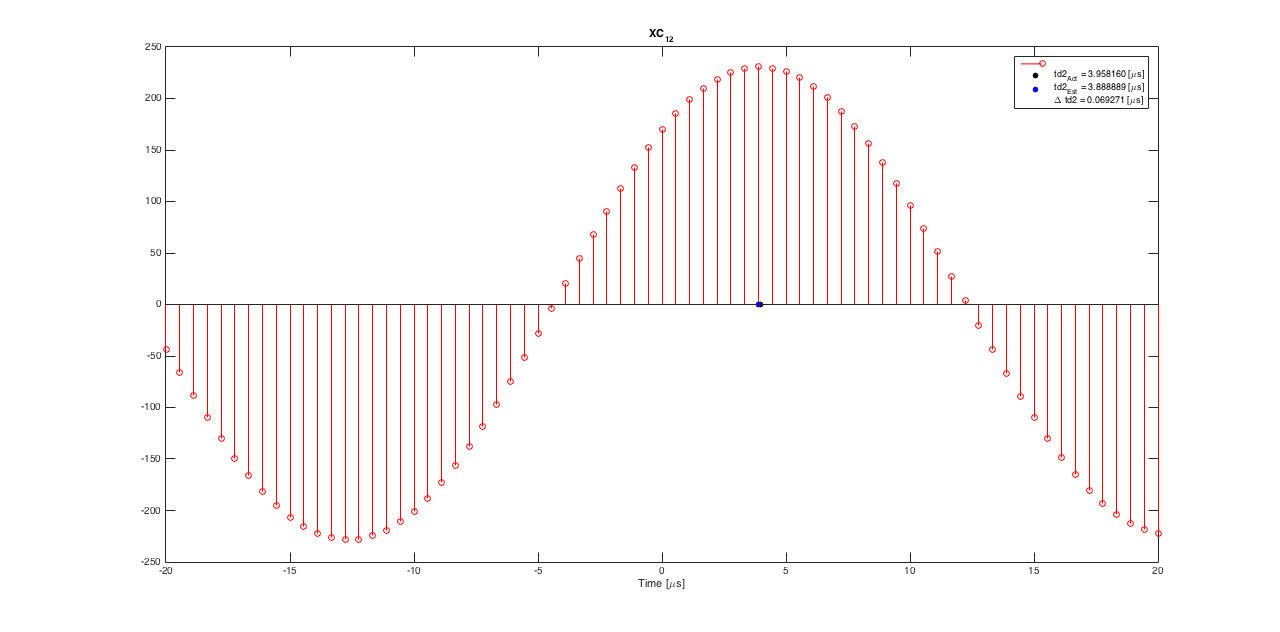
\includegraphics[width=10.0cm]{/Users/betio32/Documents/myGitHub/Senior-Design/Reports/Pics_and_Figs/XC_Partial_Heads.png}
    \caption{Cross-correlation being applied to Fig. 5.} \label{fig:XC_Partial_Heads}
\end{figure}

\noindent Note that since the sensor spacing was restricted to being less than half a wavelength, the cross-correlation function yields one and only one maximum implying maximum similarity. This is the time delay (lag) between the signals captured by chan1 and chan2.

\subsection{Error Analysis for Diamond and Tetrahedron Geometries}

\noindent Both the diamond and tetrahedron TDOA geometries were simulated using MATLAB. Of principal concern to the design team was which geometry was superior in providing the least amount of error possible in the azimuth estimates.\\

\noindent The maximum theoretical error in the time delay estimations using the cross-correlation function is the sampling period ($t_s$). However, to compute the cross-correlation function involves numerical integration which introduces rounding error, underestimation, and overestimation. The more realistic error in the time delay estimate is more likely $2t_s$. To minimize the error a number of numerical integration techniques were explored: Simpsons Rule, Midpoint Rule, and the Trapezoidal Rule. Of these methods the Trapezoidal Rule yielded the least amount of error. The Romberg Method may be explored in the future if deemed necessary. 

\pagebreak

\begin{figure}[!h]
	\centering
	\begin{subfigure}{.5\textwidth}
  		\centering
  		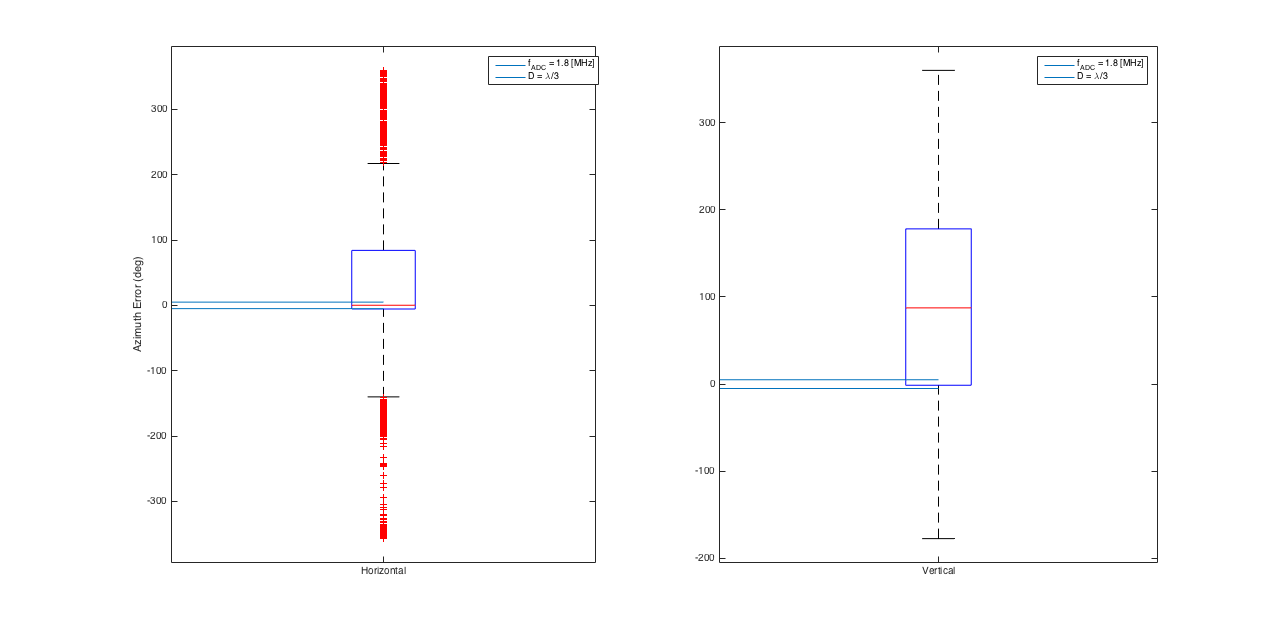
\includegraphics[width=.85\linewidth]{/Users/betio32/Documents/myGitHub/Senior-Design/Reports/Pics_and_Figs/Error_Analysis_Diamond_Third.png}
  		\caption{Diamond geometry.}
  		\label{fig:Error_Analysis_Diamond_Third}
	\end{subfigure}%
	\begin{subfigure}{.5\textwidth}
  		\centering
  		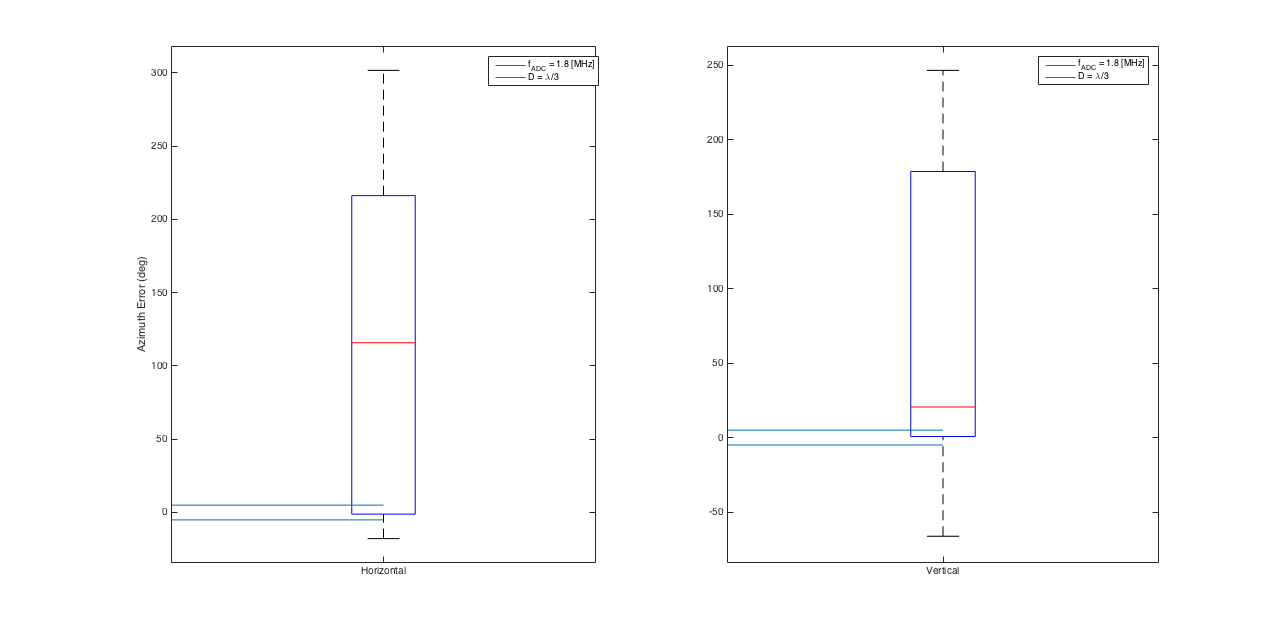
\includegraphics[width=.85\linewidth]{/Users/betio32/Documents/myGitHub/Senior-Design/Reports/Pics_and_Figs/Error_Analysis_Tetra_Third.png}
  		\caption{Tetrahedron geometry.}
  		\label{fig:Error_Analysis_Tetra_Third}
	\end{subfigure}
	\caption{Azimuth error analysis for $D=\frac{\lambda}{3}$.}
\end{figure}

\noindent As can be seen in Fig. 7, the azimuth error analysis showed huge variation. This was a major problem that had to be overcome.\\

\noindent Of interest to the design team was pinpointing the cause of the inconsistency.

\begin{figure}[!h]
	\centering
	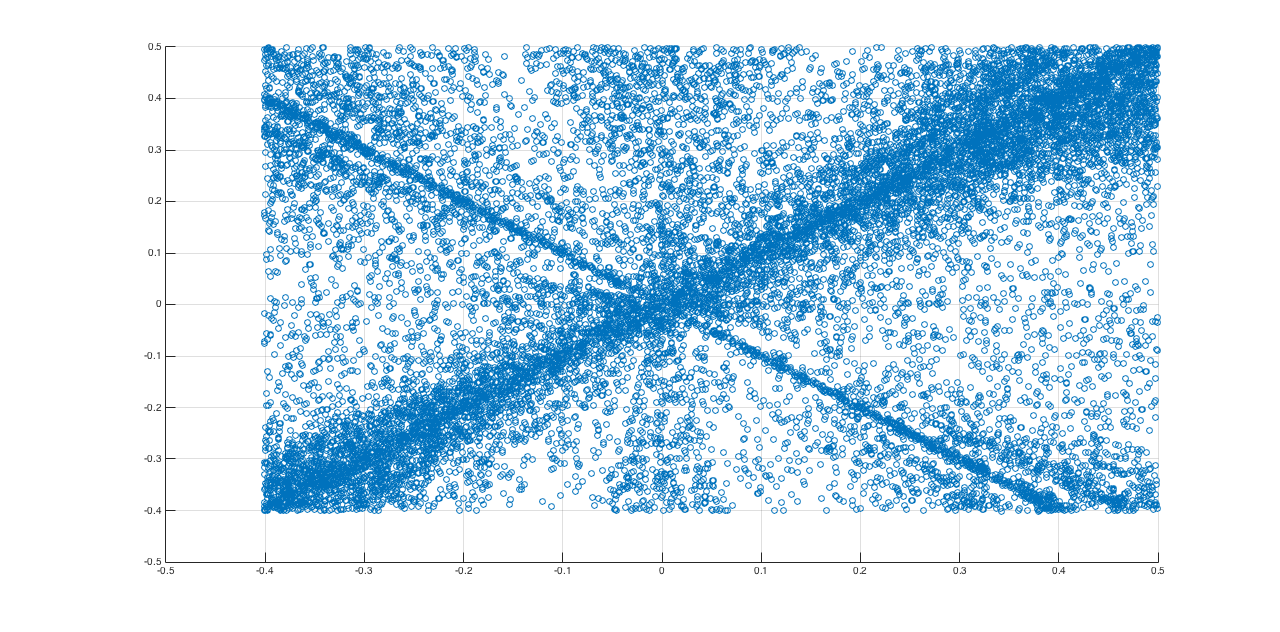
\includegraphics[width=10.0cm]{/Users/betio32/Documents/myGitHub/Senior-Design/Reports/Pics_and_Figs/Diamond_Dead_Zones.png}
    \caption{Diamond geometry dead zones.} \label{fig:Dimaond_Dead_Zones}
\end{figure}

\noindent In Fig. 8, a statistical analysis was conducted on the diamond geometry for 100E+3 trials. The pinger location was randomized using a normal distribution. If the solution to the estimated pinger location was complex, then the actual pinger location was plotted in a 3D scatter plot. The analysis shows "dead zones" along the NE,SE,SW, and NW directions. This is caused by the pressure wave reaching two sets of pairs of hydrophones at the same time. 

\pagebreak

\subsection{Increasing the Sensor Spacing Beyond Half a Wavelength}

\noindent Due to the error analysis that was depicted in Fig. 7, the design team tried to increase estimated azimuth consistency by increasing the sampling rate of the Analog-to-Digital-Converter (ADC). Error was not satisfactory until the ADC frequency was in the several GHz.\\

\noindent The solution came by the suggestion of increasing the sensor spacing beyond half a wavelength as depicted in Fig. 9. The diamond configuration showed a significant decrease in error while the tetrahedron did not. This would suggest that if the prototype footprint is desired to be small, then the diamond geometry would be more favorable than the tetrahedron geometry. 

\begin{figure}[!h]
	\centering
	\begin{subfigure}{.5\textwidth}
  		\centering
  		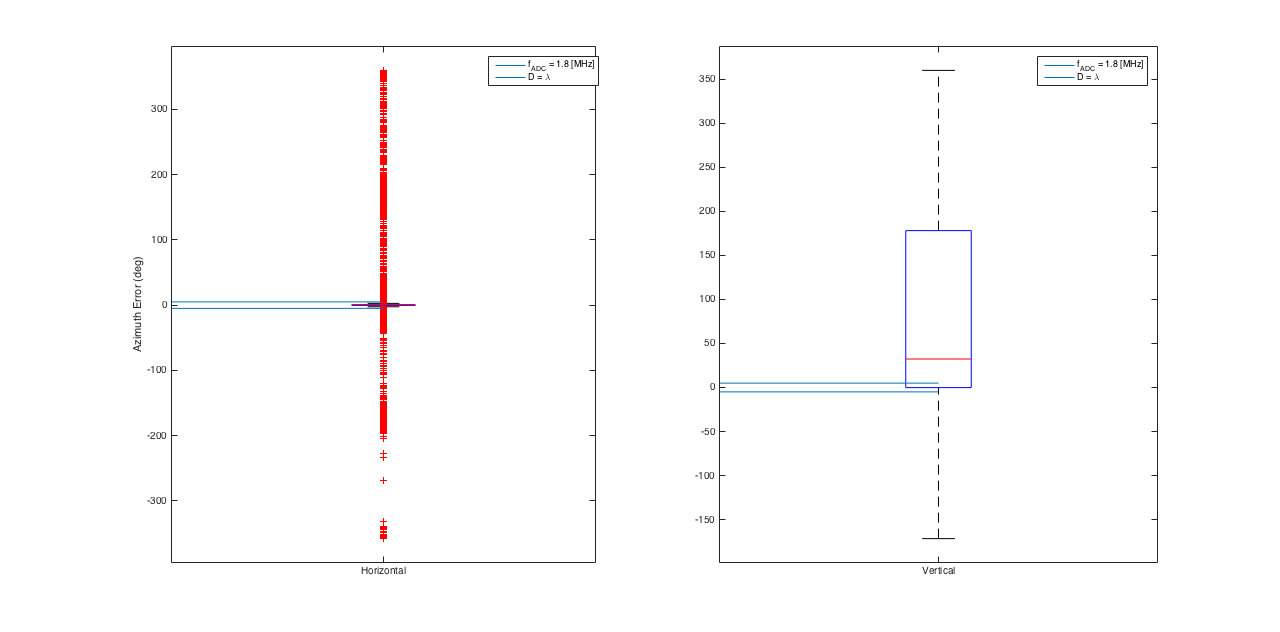
\includegraphics[width=.85\linewidth]{/Users/betio32/Documents/myGitHub/Senior-Design/Reports/Pics_and_Figs/Error_Analysis_Diamond_One.png}
  		\caption{Diamond geometry.}
  		\label{fig:Error_Analysis_Diamond_One}
	\end{subfigure}%
	\begin{subfigure}{.5\textwidth}
  		\centering
  		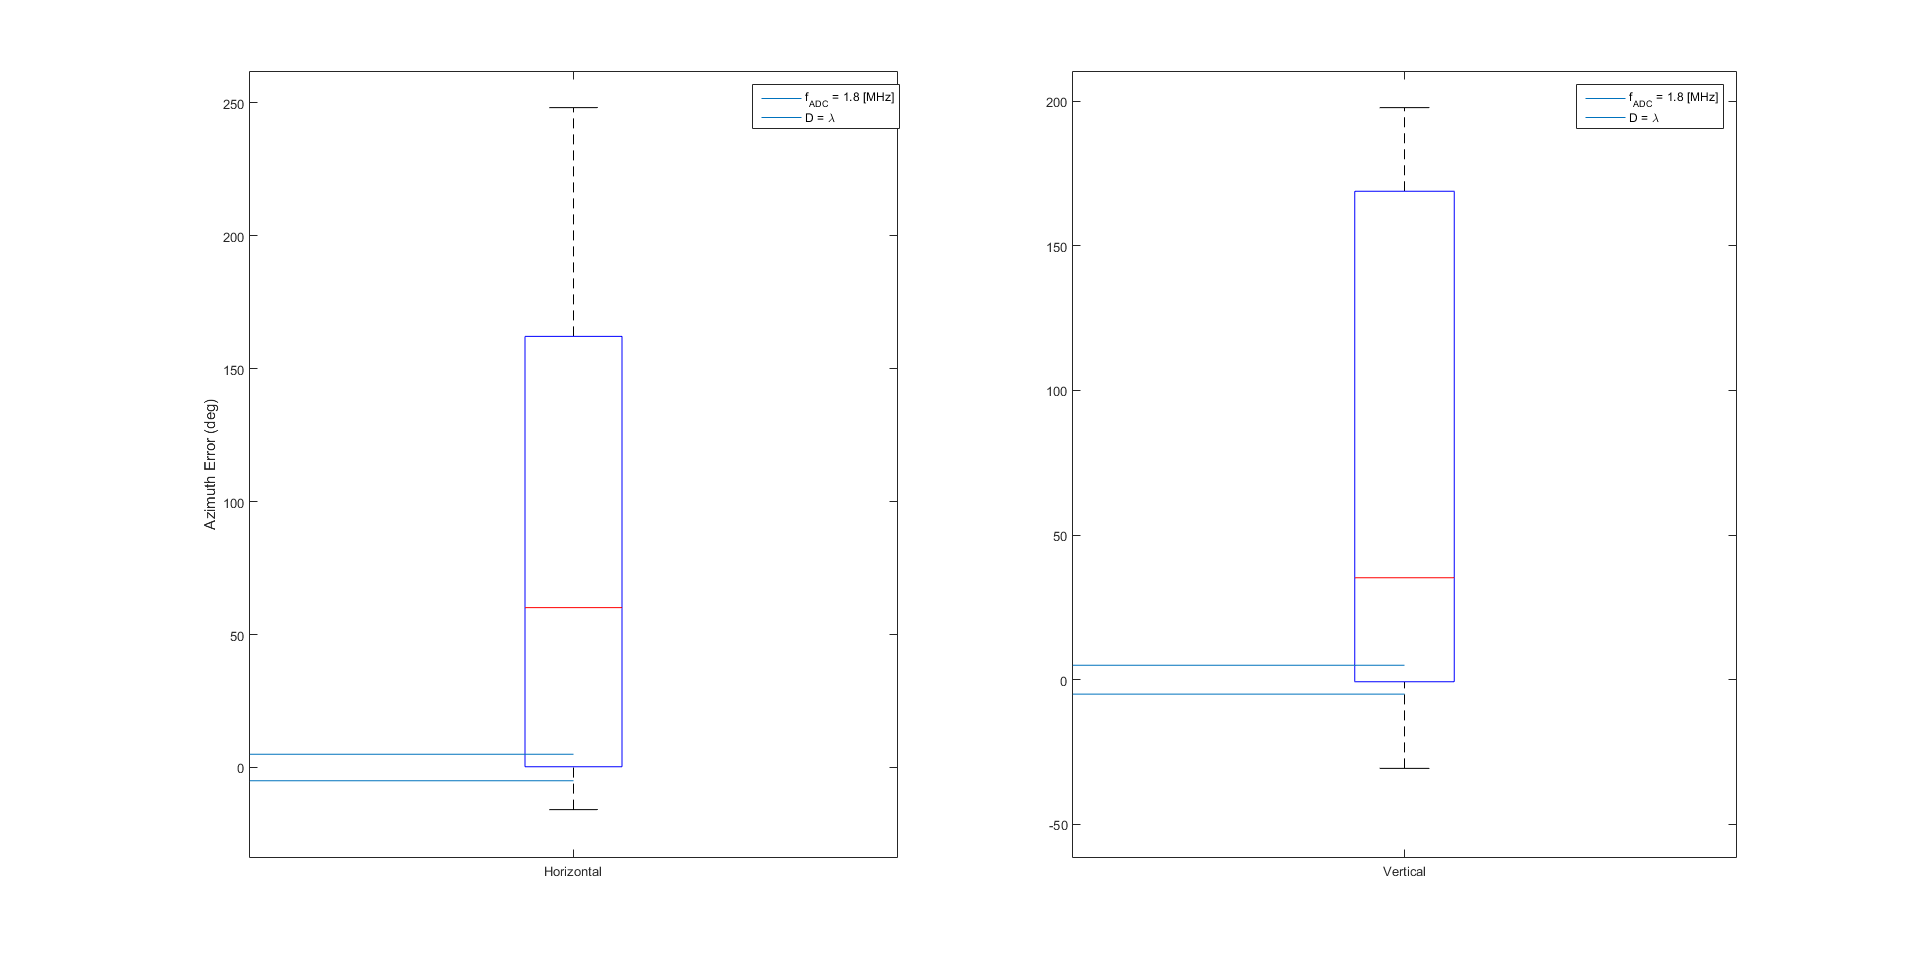
\includegraphics[width=.85\linewidth]{/Users/betio32/Documents/myGitHub/Senior-Design/Reports/Pics_and_Figs/Error_Analysis_Tetra_One.png}
  		\caption{Tetrahedron geometry.}
  		\label{fig:Error_Analysis_Tetra_One}
	\end{subfigure}
	\caption{Azimuth error analysis for $D=\lambda$.}
\end{figure}

\noindent However another problems arises as a result of the increased sensor spacing. The cross-correlation functions now contain multiple maximums as depicted in Fig. 10. The peak-of-interest (POI) can be determined by calculating secondary time delays.\\

\noindent Refer to Fig. 5. We see that chan1 received the signal first at approximately 280 $\mu$s while chan2 received the signal a little while later at approximately 290 $\mu$s. The estimated time delay for chan2 is then about 10 $\mu$s. We compare this secondary time delay to the peak locations for the cross-correlation function in Fig. 10. We see that the closest peak to 10 $\mu$s is at 5 $\mu$s. This is the POI!

\pagebreak

\begin{figure}[!h]
	\centering
	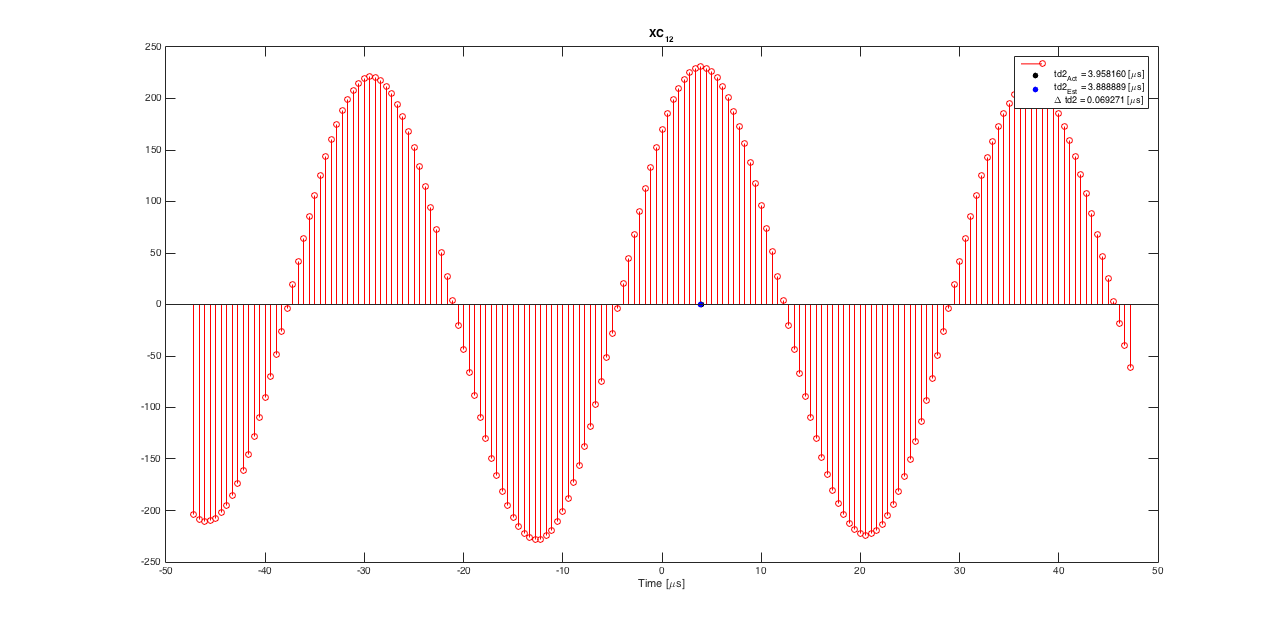
\includegraphics[width=10.0cm]{/Users/betio32/Documents/myGitHub/Senior-Design/Reports/Pics_and_Figs/XC_Full_Heads.png}
    \caption{Cross-correlation with multiple maximums from $D \geq \frac{\lambda}{2}$.} \label{fig:XC_Full_Heads}
\end{figure}

\subsection{Memory Limitation and the Need for an External Trigger}

\begin{figure}[!h]
	\centering
	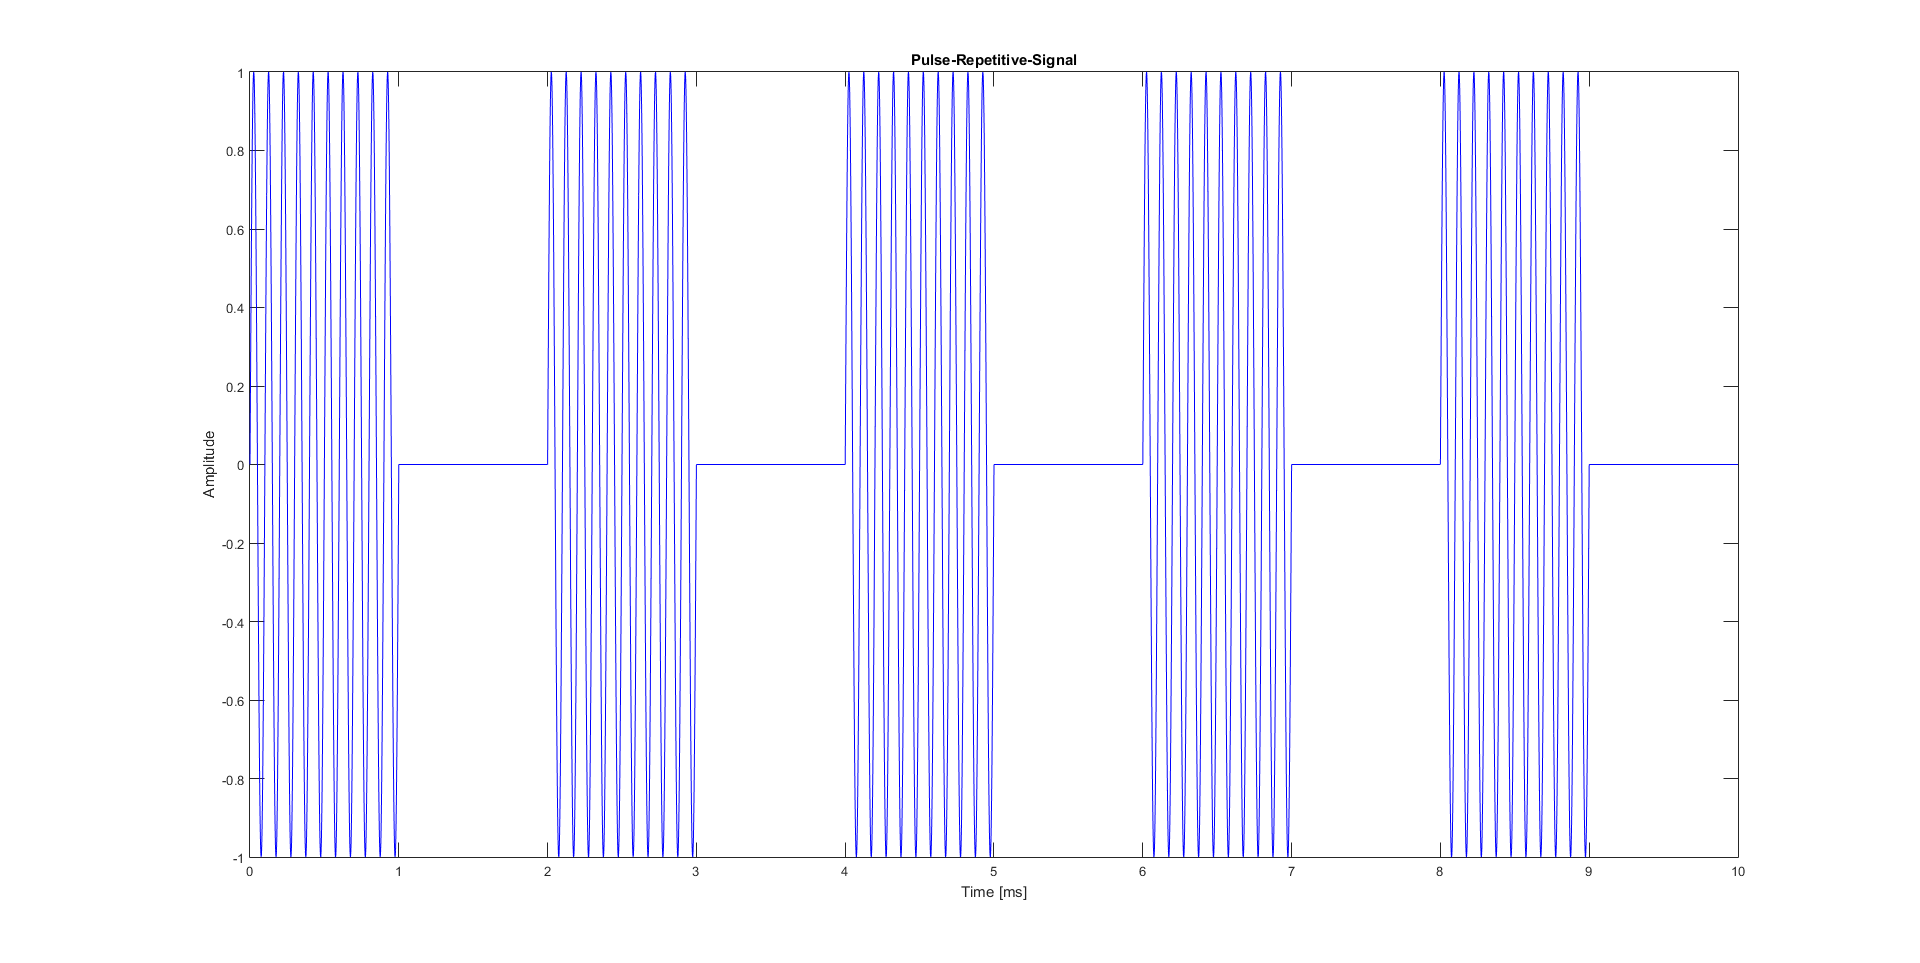
\includegraphics[width=10.0cm]{/Users/betio32/Documents/myGitHub/Senior-Design/Reports/Pics_and_Figs/Pulse_Repetitive_Signal.png}
    \caption{Example pulse-repetitive-signal.} \label{fig:Pulse_Repetitive_Signal}
\end{figure}

	Number of samples required to capture a complete PRT. 
    Using a 555 Timer for pulse detection.

\pagebreak

\begin{figure}[!h]
	\centering
	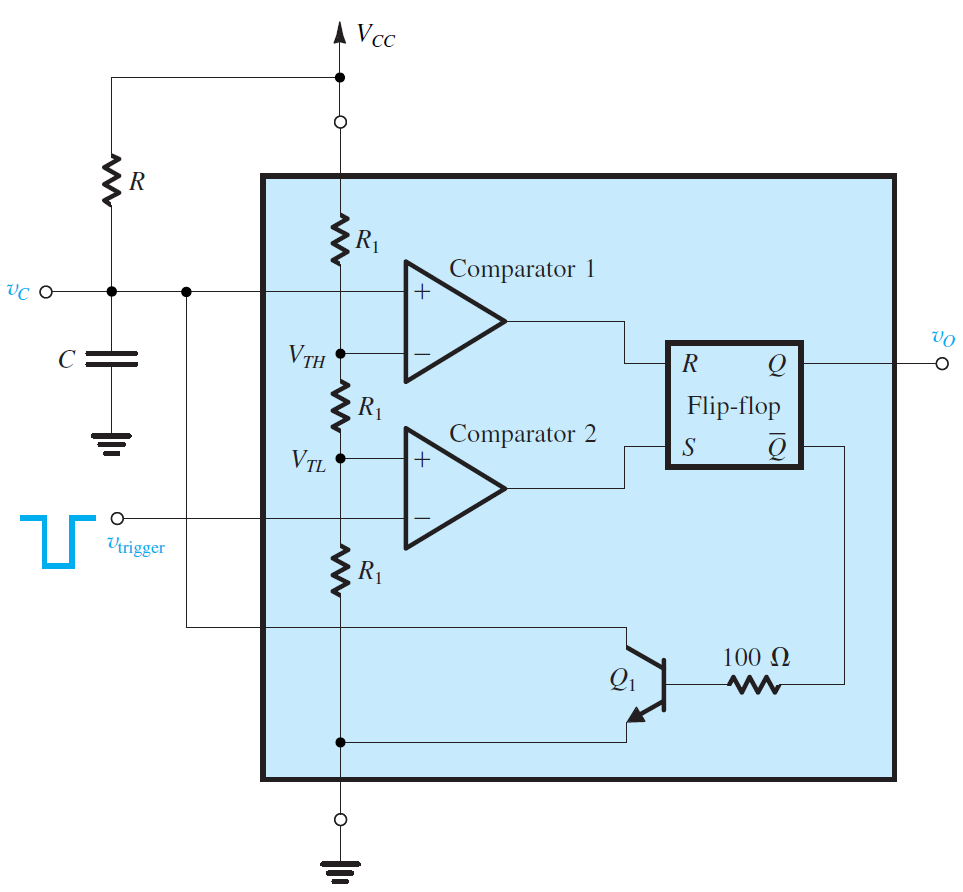
\includegraphics[width=10.0cm]{/Users/betio32/Documents/myGitHub/Senior-Design/Reports/Pics_and_Figs/555_Timer.png}
    \caption{Trigger based off 555 timer.} \label{fig:555_Timer}
\end{figure}

\subsection{Determining the Time Delays from the Tails}

\section{Implementation}

\subsection{Digital Signal Processing Desired Parameter Values}
	N0 = 1024 or 2048 for higher XC resolution for increased precision and accuracy of time delay estimations.
    
    FFT
    	Importance that it be a power of 2 for FFT acceleration.
    	Divide and conquer

\subsection{Analog and Digital Filter Placement}
	No analog filter between ADC and FPGA because of phase distortion.
    Response time of analog filter for trigger.

\subsection{Other Considerations}
	PCB Layout
    	-Transmission Lines
        -Number of layers required

	Creating a memory buffer inside the FPGA for uninterrupted sampling.
    
    The need for H/W accelerated FFT and if DSP libraries will be available.
    
    Xilinx Zynq 7000 SoC. ARM micro-controller and an FPGA on the same chip.

\end{document}

%----------------------------------------------------------------------------------------
%	END OF DOCUMENT
%----------------------------------------------------------------------------------------